\documentclass[a4paper]{article}
\usepackage{natbib,alifeconf}

\usepackage{subfig}
\usepackage{xcolor}
\usepackage{fancybox}




\title{Bootstrapping the Support Vector Machine}

\author{Thomas Goerttler$^{1,2,3}$, Christian Koopmann$^{1,2,3}$, Patricia Craja$^{1,2,3}$ \\
\mbox{}\\
$^1$Humboldt University of Berlin, Unter den Linden 6, 10099 Berlin \\
$^2$Free University of Berlin, Kaiserswerther Str. 16-18, 14195 Berlin \\
$^3$Technical University of Berlin, 10623 Berlin \\
thomas.goerttler@gmail.com\\
c.k.e.koopmann@gmail.com\\
Patricia.craja@gmx.de\\
}


\begin{document}
\maketitle


\begin{abstract}
The goal of this project is the analysis of the variance of Support Vector Machines (SVMs) and the relationship between this variance and other important aspects of the SVM. We provide a characterization of the variance of SVMs using the minimal distance of prediction points to the decision boundary and apply the bootstrap method in order to estimate the uncertainty of the prediction rule. Therefore we use parallelization. Finally it will be showed how the variance is correlated with other characteristics of the SVMs, such as the regularization parameter and the number of support vector machines, as well as how the balance of the training data set influences the variance. This impact is analyzed for both Linear and Gaussian Kernel SVMs. Doing this for simulated data as well as real data similar results are obtained and we concentrate in this paper on showing the results obtained for the simulated data. 
  
\end{abstract}

\section{Introduction}

Support Vector Machines are one of the most successful methods of Machine Learning (\cite{steinwart_support_2008}). SVMs have many merits that distinguish them from many other machine learning algorithms, including the nonexistence of local minima, the speed of calculation, and the use of only two tuning parameters. Given a binary training data set, an SVM learning algorithm builds a model that predicts the unknown class for new input data, making it a non-probabilistic binary linear classifier (\cite{cristianini_introduction_2000}). SVM is based on a minimization problem, which seeks for a hyperplane in the feature space that optimally separates data points of two clusters.  By reducing non-linear complex decision problems to linear problems through application of the Kernel-Trick, they represent a computationally efficient way to tackle these problems. The dimension of the feature space is controlled by the choice of a specific Kernel function. Common Kernels are the Linear Kernel, the Gaussian Kernel (RBF) and the Polynomial Kernel.

SVMs based on certain Kernels (e.g. Gaussian RBF Kernel) are non parametric methods. Since the distribution of the underlying data is generally unknown, so is the finite sample distribution of these methods (\cite{hastie_elements_2005}).

There has been considerable research on the asymptotic distribution of SVMs, which have been shown to be asymptotically normally distributed under certain conditions. An alternative idea to estimate these distributions is to use Efrons empirical bootstrap (\cite{efron_introduction_1994}). The idea behind this method is to repeatedly draw samples with replacement from the full data according to the empirical distribution function of the data. Through the repeated calculation of the statistic of interest one can get an estimate of its distribution. For the SVM this estimate has been shown to be consistent under relatively mild conditions.
    
In the first section we will give an overview of the Problem to calculate the variance of the SVM. Then we will explain how we implemented the Bootstrap and the Data Simulation in order to estimate this variance. Once we estimated the variance we can finally analyze the influence of different parameters on this variance for both Linear and Gaussian Kernels.

\section{Problem}
In contrast to probabilistic classifiers which provide classification with a degree of certainty, SVMs only predict the most likely class that the sample should belong to.  

Since no adequate distribution theory exists, we provide bootstrapping method to the SVM algorithm, i.e. drawing random training samples with replacement from the full training data set to train different SVMs. Through the repeated calculation of the predictions of the test data set we can estimate the prediction variance, which is an indicator of the degree of certainty of the SVM. 

Predictions are only binary variables. Therefore might be identical across all bootstrap samples we use real valued substitutes such as the minimal distance of each prediction point to the decision boundary (figure \label{fig1}) or the probability of each prediction point to belong to the predicted class. After testing both substitutes we decided to use the minimal distance to the decision boundary as it turns out to be a better indicator for the prediction variance, so our examples will be based on that. 


\begin{figure}[!htb]
\begin{center}
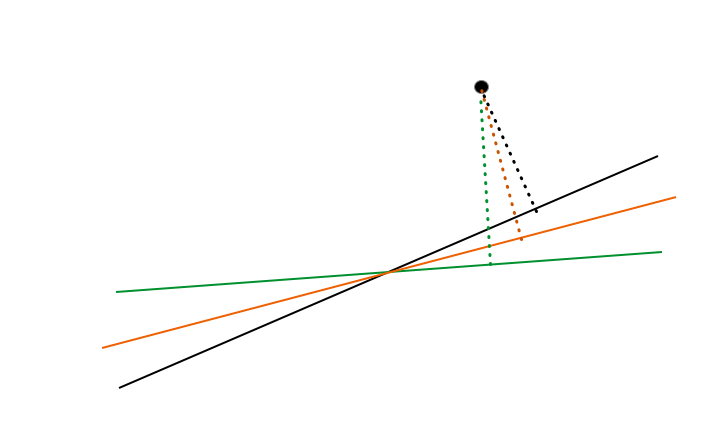
\includegraphics[width=2.5in]{abb/distances.jpg}
\caption{The minimal distance of a prediction point to each hyperplance is considered.}
\label{fig1}
\end{center}
\end{figure}




\section{Implementation}

\subsection{Bootstrapping}
In order to calculate the variance of the predictions we use bootstrap samples. We start by training the SVM on the full training data and will call this SVM the \textit{Full SVM}. Then we draw $N$ random bootstrap samples with replacement (\cite{christmann_bootstrap_2013}) from the full training data and train the SVM $N$ times on each bootstrap sample in a parallelized manner. That way we get $N$ different SVMs that predict for each input of the test data of size $n$ to which class it belongs. In figure \label{fig2} the difference in the hyperplanes in the linear can be seen. If the data is perfectly seperated (in a and c) than the variance is smaller than if the data cannot perfectly seperated. It is also seen, that the variance is smaller if the training data do have more observations.

The $n$ distances of each point in the test data set from the decision boundary can be seen as a random variables. For the $N$ SVMs we obtain $N$ different values of these random variables and can calculate their variance. We take the average of these $n$ variances as an indicator for the variance of the \textit{Full SVM}. Therefore our Bootstrap Method uses as input the training data set, the test data set, SVM-Parameters, and the number $N$ of bootstrap replications and it returns the \textit{Full SVM}, its number of support vectors as well as its variance.


\begin{figure}[!htb]
\begin{center}
\subfloat[Var: 0.20950]{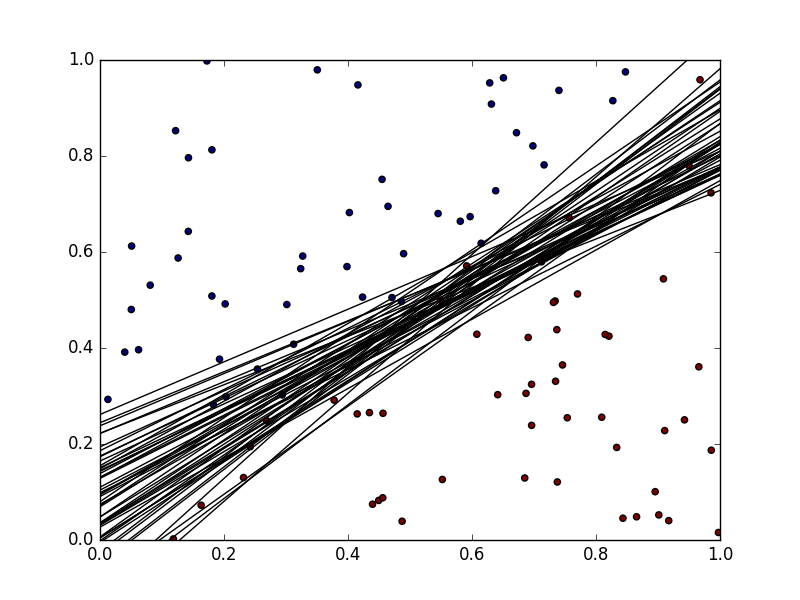
\includegraphics[width=1.5in]{abb/100_n.jpg}}
\subfloat[Var: 0.26697]{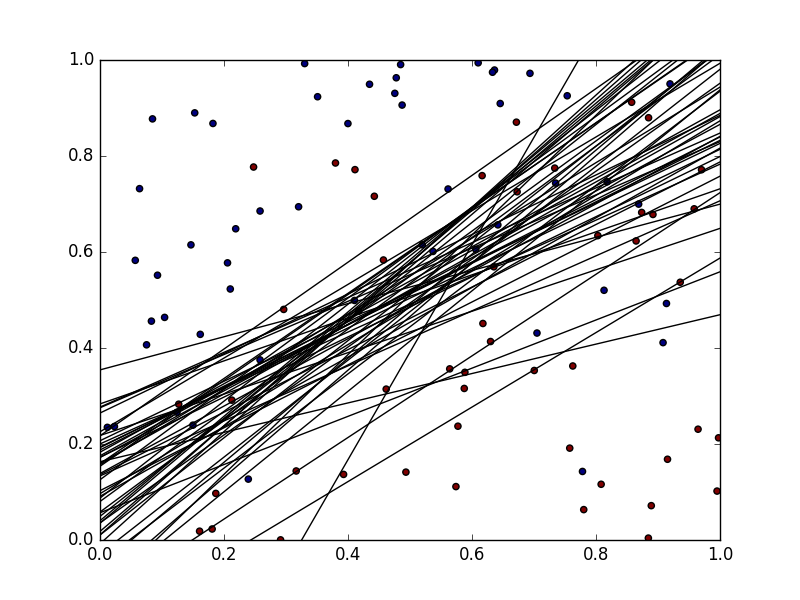
\includegraphics[width=1.5in]{abb/100_y.jpg}}

\subfloat[Var: 0.12684]{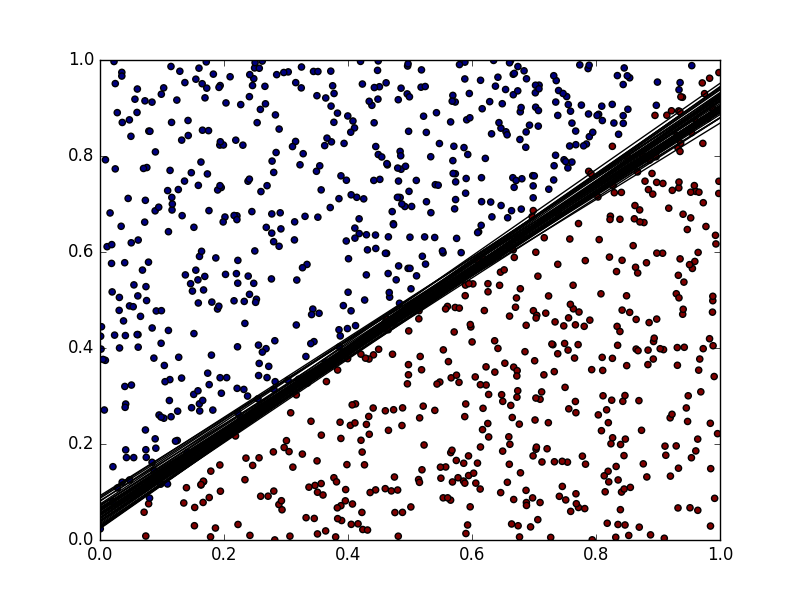
\includegraphics[width=1.5in]{abb/1000_n.jpg}}
\subfloat[Var: 0.15181]{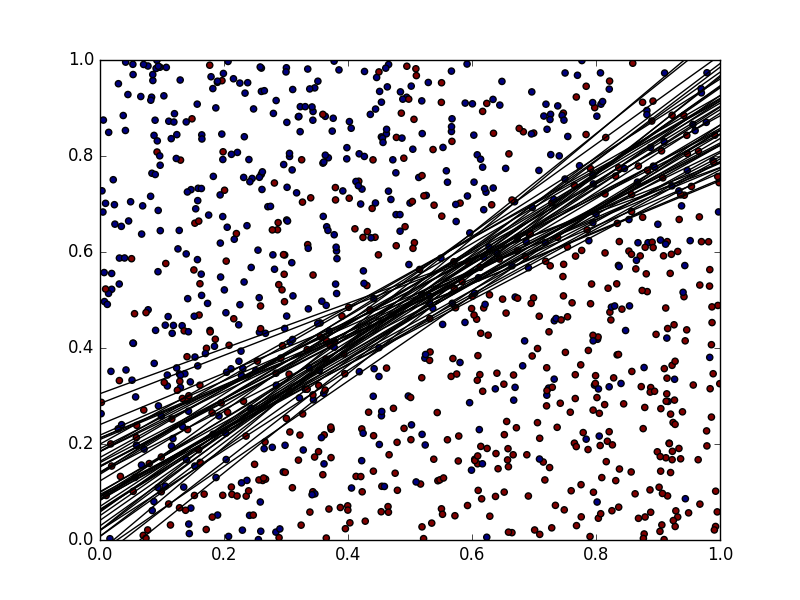
\includegraphics[width=1.5in]{abb/1000_y.jpg}}
\caption{In each picture 100 hyperplances are plotted based on samples. In (a) and (c) the data are perfectly seperated wheareas in (b) and (d) small errors occur. In (a) and (b) the trainig data have 100 observations in (c) and (d) 1000.}
\label{fig2}
\end{center}
\end{figure}

\paragraph{Parallelization:} In order to make the bootstrapping efficient, it is parallelized. A pool of processes is created which carry out tasks submitted to with the Python \texttt{Pool} class it. Each process does the bootstrapping parallely and independent of the other processes. The important results of each SVM are written back to an array.

\subsection{Data Simulation}
For the Data Simulation we use two different approaches, the Hyperplane- and the Centroid- Approach. For both we assume to randomly draw $n$ observations for the input variables $x$ from a normal distribution. The Hyperplane-Approach calculates the labels using the formula $y= sign(c+ w^T x + error)$, given the Hyperplane parameter $w$, a constant $c$ as well as the error distribution, whereas the Centroid-Approach calculates the labels using the formula $y= sign(c + a_1*(d(x,z_1)^{-1}... + error)$ given the Centroid- Locations $z_i$, the Centroid- Parameters  $a_i$, a constant $c$ and a distance function $d(a,b)$.
Two change the number of support vectors of a data set the variance of the error must simply be higher. To change the balance of the data set, the intercept is to be changed.


\section{Results}

In this section we will show how the prediction variance is correlated with other aspects of the SVM, such as the regularization parameter $C$, the balance of the training data set and the number of support vectors of the original Full-SVM. Analyzing this impact for both Linear  and Gaussian Kernel SVMs we found following interesting results:

\begin{figure}[!htb]
\begin{center}
\subfloat[]{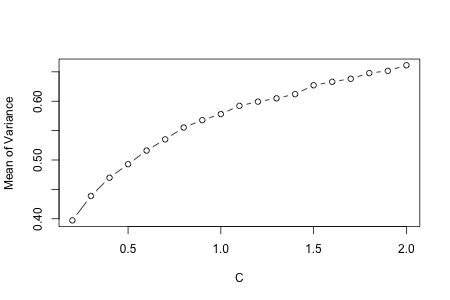
\includegraphics[width=3in]{abb/c_lin.jpg}}

\subfloat[]{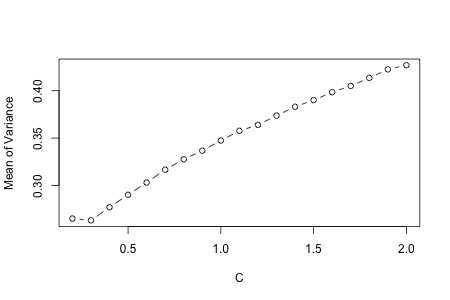
\includegraphics[width=3in]{abb/c_rbf.jpg}}
\caption{The results for changing the regularization parameter $C$. On the y-axis the mean of the variance of 20 different datasets for each $C$ is seen. Each datasets has 100 overservations and 1000 replications are done. (a) shows the result for the linear kernel, (b) for the gaussian.}
\label{fig3}
\end{center}
\end{figure}



\subsection{Influence of the regularization parameter C}
\paragraph{Observations:}
As it is seen in figure \label{fig3}, changing the regularization parameter $C$ we obtained similar results for both Linear and Gaussian Kernel SVMs. The higher we choose our regularization parameter $C$, the higher will be the variance of the SVM. The parameter $C$ is therefore positively correlated with the variance.
\paragraph{Explanation:}
The parameter C controls the trade off between errors of the SVM on training data and margin maximization. To avoid overfitting, the SVM employs regularization and controls the amount of regularization by the constant $C$ (\cite{hastie_elements_2005}). A high value of $C$ corresponds to low regularization, i.e. lower size of slack variables and therefore higher overfitting, which means that the SVM fits the training data too well but does not generalize to new data and therefore the variance of the predictions of our test data rises.

Figure 6 shows this relation for values between 0 and 2 of the parameter $C$ 
for Linear and Gaussian Kernels. Because each value of $C$ corresponds to a different \textit{Full SVM}, we calculated the average of 20 SVM variances for each value of C, i.e. 20 test data set variances as explained at the beginning (using $N$=1000 Bootstrap Replications, and $n$=100 data points).
 
\begin{figure}[!htb]
\begin{center}
\subfloat[]{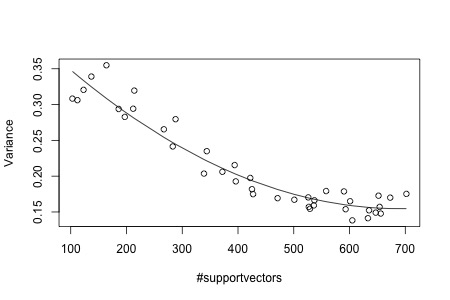
\includegraphics[width=3in]{abb/n_lin.jpg}}

\subfloat[]{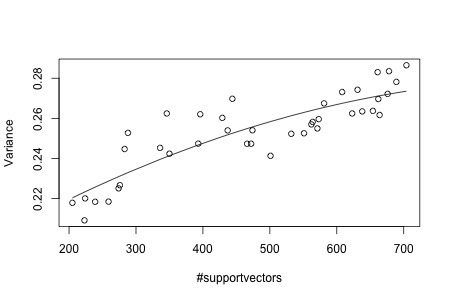
\includegraphics[width=3in]{abb/n_rbf.jpg}}
\caption{In this pictures the variance of the results for changing number of support vectors are depicted. Each dataset has 1000 observations and 500 samples are drawn. (a) shows the result for the linear kernel, (b) for the gaussian.}
\label{fig4}
\end{center}
\end{figure}


\subsection{Influence of the number of support vectors}
\paragraph{Observations:}
In figure \label{fig4} it can be seen, that thanging the number of support vectors for the \textit{Full SVM} we obtain different results for Linear and Gaussian Kernels. For the Linear Kernel, the variance of the SVM gets smaller with more support vectors, whereas for the Gaussian Kernel the variance rises with more support vectors. The number of support vectors is therefore negatively correlated with the variance of the Linear Kernel and positively correlated with the variance of the Gaussian Kernel.
\paragraph{Explanation:}
The number of support vectors controls the slack variables of the soft margin SVM. A high number of support vectors implies larger margins and higher slack variables. Training the Linear SVM on the bootstrap samples is therefore more robust and the variance of the decision boundary as well as the distance from each point of the test data set to the decision boundary has smaller variation.
For Gaussian Kernels, a higher number of support vectors implies overfitting on the training data set and does not generalize well to new data and therefore the variance of the predictions of our test data rises.

\begin{figure}[!htb]
\begin{center}
\subfloat[]{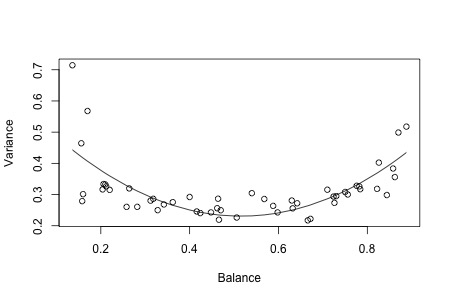
\includegraphics[width=3in]{abb/bal_lin.jpg}}

\subfloat[]{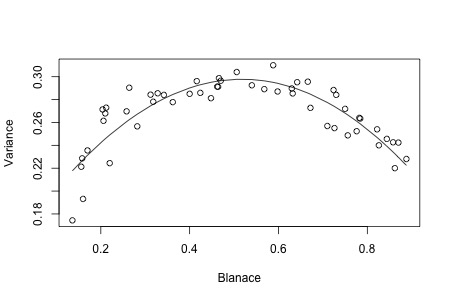
\includegraphics[width=3in]{abb/bal_rbf.jpg}}
\caption{In the figures the variances are shown dependet on the balance of thre data. Each dataset has 500 observations and 1000 samples are drawn (a) shows the result for the linear kernel, (b) for the gaussian.}
\label{fig5}
\end{center}
\end{figure}


\subsection{Influence of the balance of the training dataset}

\paragraph{Observations:}
Changing the balance of the tranings data set, from which the samples are taken, we obtain different results for the Linear and Gaussian Kernels, as it is seen in figure \label{fig5}. But for both the behaviour is symmetric. For the Linear Kernel, the variance of the SVM is higher when the data are unbalanced. His variance is smallest when the data is perfectly balanced, so 50 \% of the data have label $1$ and the other part has $-1$. However, for the Gaussian Kernel the variance is the highest when the data is perfectly balanced. 
\paragraph{Explanation:}
In the linear case the variance is especially high, when one class is really small compared to the other class. The linear hyperplance is really dependent of the few points from the small class according to which points are take from this class, the difference of the hyperplance can be massive.
The Gaussian kernel shows exactly the different results. This occurs because the Gaussian Kernel tends to overfit the data on the trainings sets (\cite{hastie_elements_2005}). We have taken 1000 samples from the data set. If the data are perfectly balanced, there are more possible different samples of the smaller group possible. Therefore the hyperplance differ more. If the smaller class is really small, the sample from the smaller class can not differ that much from each other.
Nevertheless it can be obtained, that the effect is extremly high in the tails and between a balance of 0.3 to 0.7 is cannot really be said that the effect already occurs.


\section{Conclusion}

Calculating the variances by using bootstrap samples seem to be a quite good idea to calculate a variance. The variance are a good indicator for the robustness of the SVM as in figure \label{fig2} can be seen.
The results for changig the $C$-parameter are not surprising but confirm the strengh of the variance estimator.
It is really surprissing that the results of the two kernels differ so much when changig the number of support vectors and the balance of the data, are so clear, but the occurence does make sense.

\section{Outlook}

Further analysis which can be interesting in this project are to look for the influence of the dimensionality on variances. Furthermore other tuning parameter as the gamme of the rbf-kernel, the degree of polynomial kernel can be interesting. 


\footnotesize
\bibliographystyle{apalike}
\bibliography{sample}



\end{document}
